\section{Engine}
\label{verwendung_engine}

\subsection{Einbindung der FM3D-Engine}
Falls ein Projekt ohne den FM3D-Designer erstellt wird, so muss die FM3D manuell eingebunden werden. 

\subsection{Voreinstellungen}
Zunächst müssen sie die OpenGL, FreeImage, FreeType und Assimp in das Projekt einbinden. Die FM3D-Engine wird automatisch eingebunden.
$$Configuration Properties->C/C++->Additional Include Directories$$\cref{include}
$$Configuration Properties->Linker->Additional Include Directories$$
\cref{liblib}

\begin{figure}
	\begin{center}
		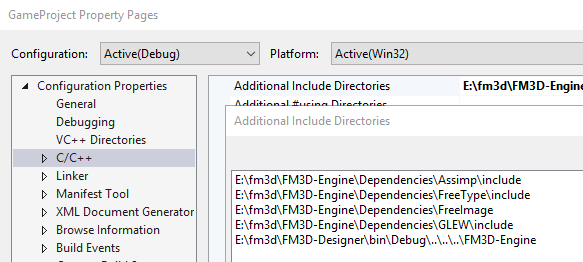
\includegraphics[width=\textwidth]{04verwendung/Engine/include.png}
		\caption{Include Verzeichnisse}\label{includeinc}
	\end{center}
\end{figure}

\begin{figure}
	\begin{center}
		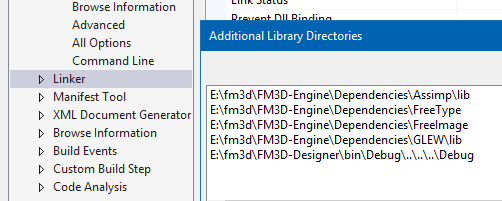
\includegraphics[width=\textwidth]{04verwendung/Engine/lib.png}
		\caption{Lib-Verzeichnisse}\label{liblib}
	\end{center}
\end{figure}

\subsection{Kamera}

\subsection{Entities}

\subsection{Inputsystem}
\label{inputsystemver}
Hierfür wird die Klasse \textit{Inputsystem} verwendet. Möchte man nun Tasten abfrage, so muss man zunächst auf die rekursive Instanz der Klasse zugreifen. 
$$FM3D::Inputsystem::GetInstance()->$$
Nun kann eine Methode aus dieser Klasse verwendet werden.
Möchten Sie nun abfragen, ob eine Taste der Tastatur gedrückt wurde, verwenden Sie die Methode
$$FM3D::Inputsystem::GetInstance()->CheckKey(int  keyid);$$
Der Integer-Wert \textit{keyid} bildet den ASCII-Code der zu abfragenden Taste ab. Die Methode gibt einen booleschen Wert zurück. Die Methode $$CheckMouse(int  keyid)$$ dient dem selben Zweck, nur wird hierbei der Status der Maus abgefragt.
Die Methode $$GetLastposClick(int keyID)$$
gibt einen zweidimensionalen Vektor vom Typ Float zurück, welcher die Position vom letzten Klick der Maus mit einer bestimmten Maustaste beschreibt. \textit{keyID} stellt die zu klickende Taste dar. 
$$GetLastposInst()$$
Die obenstehende Methode gibt Daten in Form eines zweidimensionalen Vektors mit der aktuellen Position der Maus zurück.

Alle Tasten der Tastatur und Maus können über Makros angesprochen werden. Auch können Sie die ASCII-Codes der einzelnen Tasten verwenden. Die Makros, welche die Tasten der Tastatur beschreiben starten mit \textit{"`KEY\_"'}. Die Makros, die für die Maus verwendet werden starten mit \textit{"`MAUS\_"'}.
